\documentclass[12pt,a4paper,openright,twoside]{report}
\usepackage[italian,english]{babel}
\usepackage{fancyhdr}
\usepackage{indentfirst}
\usepackage{newlfont}
\usepackage{pdfpages}
\usepackage{abstract}
\oddsidemargin=30pt \evensidemargin=20pt
\pagestyle{fancy}\addtolength{\headwidth}{20pt}\setlength{\headheight}{15pt}
\renewcommand{\chaptermark}[1]{\markboth{\thechapter.\ #1}{}}
\renewcommand{\sectionmark}[1]{\markright{\thesection \ #1}{}}
\rhead[\fancyplain{}{\bfseries\leftmark}]{\fancyplain{}{\bfseries\thepage}}
\cfoot{}
\linespread{1.3}
\begin{document}
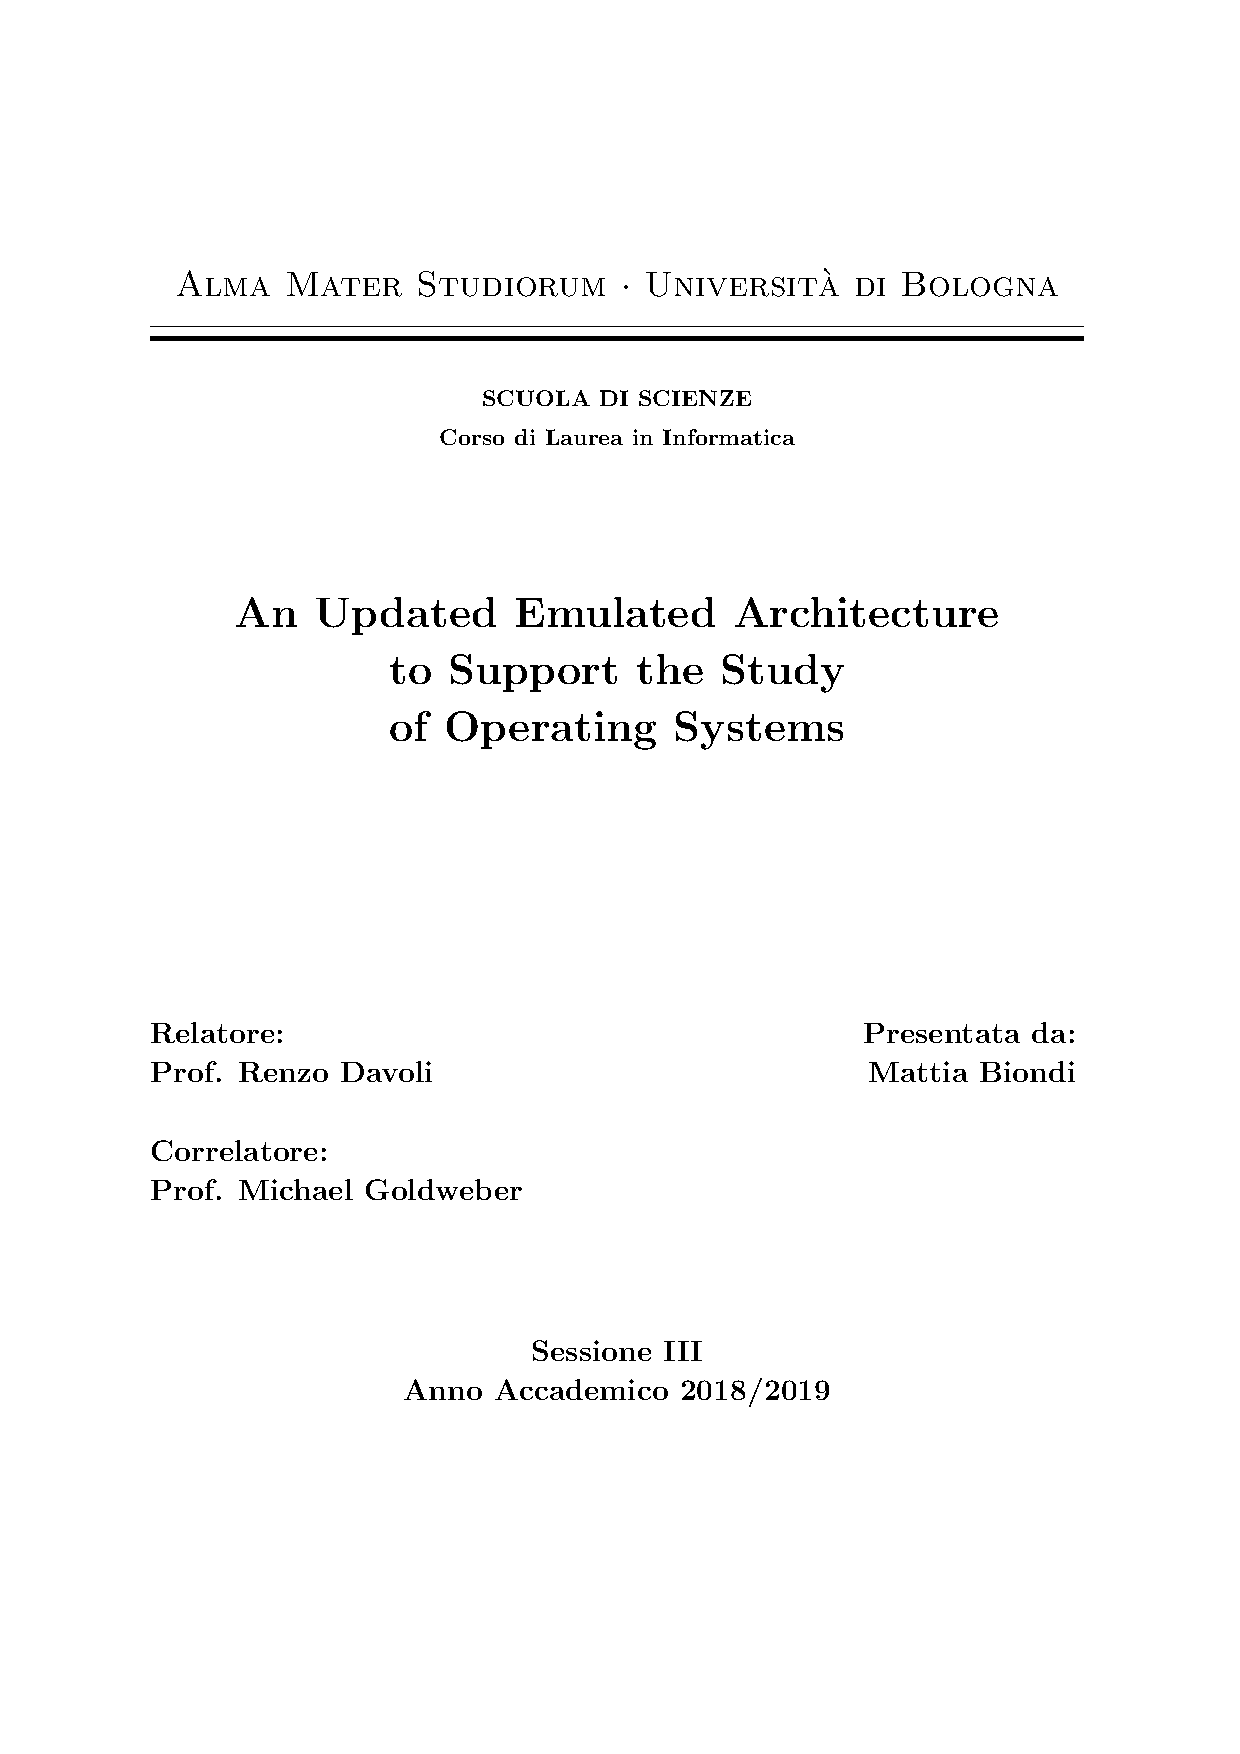
\includepdf[pages=-]{titlepage.pdf}
\clearpage{\pagestyle{empty}\cleardoublepage}
\begin{titlepage}
\thispagestyle{empty}
\topmargin=6.5cm
\raggedleft
\large
\em
Agli amici di sempre,\linebreak
alla mia famiglia,\linebreak
che non mi ha mai impedito nulla,\linebreak
e a Jas,\linebreak
senza la quale non sarei qui oggi.
\newpage
\clearpage{\pagestyle{empty}\cleardoublepage}
\end{titlepage}
\begin{abstract}
One of the most effective way to learn something new is by actively practicing it, and there is---maybe---no better way to study an Operating Systems course than by building your own OS.
It is also true that the realization of an operating system capable of running on a real hardware machine could be an overly complex and unsuitable task for an undergraduated student.
Nonetheless, it is possibile to use simplified computer system simulators in order to achieve the goal of teaching Computer Science foundations in the university environment, thus allowing students to experience a quite realistic rappresentation of an operating system.
$\mu$MPS \cite{umps} has been created for this purpose, a pedagogically appropriate machine emulator, based aroud the MIPS R2/3000 microprocessor, which features an accessible architecture that includes a rich set of easily programmable devices.
$\mu$MPS has an almost two decades old historical development and the outcome of the following thesis is the third version of the software, dubbed $\mu$MPS3.
This second major revision aims to semplify even more the emulator's complexity in order to lighten the load of work required by the students during the OS design and implementation.
Two of these semplifications are the removal of the virtual memory bit, which allowed address translation to be turned on and off, and the replacement of the tape device with a new flash drive device---certainly something more familiar to the new generation of students.
Other major improvements which concern everything from the project building tools to the front-end were made, enabling the upgrade of $\mu$MPS to a modern reliable educational software.
\end{abstract}
\clearpage{\pagestyle{empty}\cleardoublepage}
\tableofcontents
\thispagestyle{empty}
\clearpage{\pagestyle{empty}\cleardoublepage}
\pagenumbering{arabic}
\chapter{Introduction}
\lhead[\fancyplain{}{\bfseries\thepage}]{\fancyplain{}{\bfseries\rightmark}}
\chapter{TLB Floor Address}
\lhead[\fancyplain{}{\bfseries\thepage}]{\fancyplain{}{\bfseries\rightmark}}
\chapter{BIOS data structures area}
\lhead[\fancyplain{}{\bfseries\thepage}]{\fancyplain{}{\bfseries\rightmark}}
\chapter{VM bit removal}
\lhead[\fancyplain{}{\bfseries\thepage}]{\fancyplain{}{\bfseries\rightmark}}
\chapter{Flash Device}
\lhead[\fancyplain{}{\bfseries\thepage}]{\fancyplain{}{\bfseries\rightmark}}
\chapter{Project rebase}
\section{CMake}
\section{Qt5}
\lhead[\fancyplain{}{\bfseries\thepage}]{\fancyplain{}{\bfseries\rightmark}}
\chapter{Debian packaging}
\lhead[\fancyplain{}{\bfseries\thepage}]{\fancyplain{}{\bfseries\rightmark}}
\begin{thebibliography}{99}
\addcontentsline{toc}{chapter}{Bibliography}
\bibitem{umps}
  M. Goldweber, R. Davoli, and M. Morsiani,
  \textit{The Kaya OS project and the $\mu$MPS hardware emulator},
   SIGCSE Bull.,
   vol. 37, pp. 49–53,
   June 2005.
\end{thebibliography}
\end{document}
